\documentclass[%
danish,
a4paper,
onecolumn,
draftcls
]{IEEEtran}
\usepackage{EEpreamble}
\usepackage{usecases}
\newcommand{\tbd}{\textbf{\textcolor{red}{(TBD)}}}
\newcommand{\tbr}{\textbf{\textcolor{red}{(TBR)}}}
\usepackage{pdfpages}
\loadglsentries{TeX/Formalia/Ordliste}

\begin{document}

\title{
Robo-Sumo-Battle 
}
\author{
      \begin{tabular}{ll}
            Villiam Holger Bo & 201907166\\
            Adam Ryager Høj & 201803767\\
            Rasmus Kahr & 201803491\\
            David Vestergaard Kristensen & 201908226\\
            Frederik William Lassen & 201905905\\
            Daniel Schultz & 201709325\\
            Simon Fogh Thomsen & 201906472
      \end{tabular}
}
% Don't fight the engine over float placements. It's actually good at it. If you get ridiculous results it's pretty likely that your paragraphs and/or sections are too short. Try adding more text, or merging some paragraphs.

\maketitle
\tableofcontents

\printglossary[nonumberlist]
\printglossary[type=\acronymtype,nonumberlist,title=Forkortelser]
\section{Projektets mål} 

Projektets overordnede mål tager lige dele udspring i et ønske om et underholdende produkt, som i en grad kan leve videre efter semesterets afslutning såvel som gruppens fælles specifikke teknologiske interesser.
Produktets vision er et konkurrencepræget spil baseret på sumobrydning mellem to robotter i en glasmontre, hvor robotternes retning og hastighed styres på en hidtil ukendte måder – herunder analyse af lydniveauer og frekvenser som produceres af de to spillere såvel som sensorinput af andre arter.
Lyden produceres f.eks. med en blokfløjte eller simpelthen ved stemmens kraft.
Gruppens ønske om undersøgelse af teknologier indenfor analog- og digital lyd behandling indfries naturligt igennem robotternes styringsenheder og ønsket om dybere indsigt i design af software til indlejrede systemer, samt kommunikation mellem disse, indfries igennem hhv. robotterne- og controllernes system- og netværks-design.
Projektet vil yderligere bibringe en stor læring om aktuatorer, mere specifikt motorstyring, som vil være en central del af projektet.

Foruden de faglige mål for læring ønsker gruppen at styrke kendskabet til Scrum som vil anvendes til at styre en iterativ arbejdsproces, som adskiller sig fra processen kendt fra tidligere semestre. 


\figOC{Formalia/RigtBillede.png}{0.8}{Rigt billede der viser hvordan produktet er tiltænkt.}
\section{Koncept}
 Kender vi ikke alle problemet med en drukmås der har drukket for mange øller og får lyst til at skrige i en mikrofon? Det hidtil eneste kendte produkt til at afhjælpe dette problem, har været karaoke, dog med den ulempe at alle andre på baren skal høre på det. Robo-Sumo-Battle vil specifikt afhjælpe dette problem ved i stedet at lade personen bruge sin stemme til at styre to små chubby robotter der dyrker sumo-brydning, som samtidig er sjov at se på - vi bruger således en gammel japansk tradition til at afhjælpe problemerne med en nyere japansk tradition. 

Produktet er et spil for to spillere, hvor hver spiller styrer en to-hjulet robot rundt på en bane.

Styringen foregår via én kontrolenhed pr. spiller og vil være baseret på sensorinput i form af lyd igennem en mikrofon og bevægelse igennem et \textit{d-pad}. Dertil kan man aktivere forskellige \textit{gamemodes} hvor der er udviklet mere eller mindre arbitrære styringer for at skrue sværhedsgraden op. 
Disse signaler bliver digitalt behandlet og sendt til robotterne som styrekommandoer via den embedded software i spilplatformen.
Spillet er tænkt udført som en traditionel japansk sumokamp --- de to robotter mødes i en ring og kæmper. Vinderen er den robot med flest liv efter endt tid - eller den sidste robot i ringen.

\subsection{Spilregler} \label{Spilregler}

\begin{itemize}
    \item De to robotter anbringes på et markeret \textit{startfelt}.
    \item Når robotterne er anbragt korrekt på deres startfelter, kan en nedtælling fra 3 sekunder startes ved, at begge spillere trykker på hver deres knap, hvorefter spillet går i gang.
    \item Hver robot har fra spillets start 3 liv.
    \item Hver runde vare maksimalt 1 minut.
    \item I en rundes varighed gælder:
    \begin{itemize}
        \item Hvis modstanderen skubbes udover den markerede bane, vindes hele spillet.
        \item Ved at påkøre modstanderen bagfra eller fra siden, mister modstanderen et liv.
        \item Hvis en spiller selv bringer sig udover den markerede bane, vinder modstanderen.
    \end{itemize}
    \item Ved tab af liv placeres hver robot ved deres respektive startfelt.
\end{itemize}

Til styringen af robotterne medfølger der til spillet et instrument med veldefinerede frekvensområder: en blokfløjte. Hertil også et \textit{d-pad}.
\\
 Til disse instrumenter tilknytter der sig som udgangspunkt følgende kommandoer: frem, tilbage, højre og venstre. Disse kommandoer eksekveres med udgangspunkt i \figref{Formalia/blokfloejte_noder} som følgende: 
\begin{itemize}
    \item A: Fremad
    \item B: Bagud
    \item C': Venstre 
    \item D': Højre
\end{itemize}

\fig{Formalia/blokfloejte_noder}{0.6}{}

\fig{Konceptillustrationer/Spilleplade_Topview.eps}{1}{Selve spilpladen}
\fig{Konceptillustrationer/Spilleplade_Sideview.eps}{1}{Spillepladen set fra siden}
\fig{Konceptillustrationer/Spilleplade_Frontview.eps}{1}{Spillepladen set fra den ene spillers side}


\section{Kravspecifikation for produktet}

\begin{itemize}
    \item Systemet \textbf{SKAL} indeholde embedded software.
    \item Spillebanen \textbf{SKAL} maximalt være Ø1.5 meter.
    \item Robotterne \textbf{SKAL} kunne styres trådløst.
    \item Robotterne \textbf{SKAL} maksimalt være $20 \times 20 \times 20$cm.
    \item Signalbehandling \textbf{SKAL} finde sted. 
    \item Signalbehandling \textbf{BØR} færdiggøres inden for 1 sekund.
    \item Robotterne \textbf{BØR} kunne holde til kollisioner.
    \item Robotterne \textbf{BØR} have batterilevetid til 10 min. aktivitet.
    \item Systemet \textbf{KUNNE} understøtte flere spiltilstande.
    \item Systemet \textbf{KUNNE} understøtte flere spillere.
    \item Robotterne har \textbf{IKKE} våbensystemer.
\end{itemize}
\section{Accepttestspecifikation}

\subsection{Krav stillet af ASE}
Se \tabref{ASE Krav}.
\begin{table}[]
\centering
\caption{Krav stillet af ASE}\label{tab:ASE Krav}
\begin{tabular}{c p{7cm}}\toprule
\# & \textbf{Udførsel af test} \\ \midrule
1 & Det konstateres hvorvidt systemet indeholder software indlejret på systemer som ikke er en PC (eksempelvis software på en mikrocontroller)\\\midrule
2 & Det konstateres hvorvidt en systemet gør brug af en aktuator, hvorved der forstås et element som påvirker de fysiske omgivelser, som eksempelvis en DC- eller stepper-motor \\\midrule
3 & Det konstateres hvorvidt systemets fysisk adskilte dele (eksempelvis SumoBot og Bil-kontrol) kommunikerer\\\midrule
4 & Det konstateres hvorvidt minimum et af de indlejrede systemer bruger Linux som styresystem \\\midrule
5 & Det konstateres hvorvidt minimum et PSoC komponent bruges som en del af systemet\\\midrule
6 & Det konstateres hvorvidt systemet optager og benytter data fra komponenter som reagerer på fysisk påvirkning\\\bottomrule
\end{tabular}
\end{table}

\subsection{Overordnede krav til til Robo-Sumo-Battle}

\begin{table}[]
\centering
\caption{Overordnede krav}\label{tab:Overordnede krav}
\begin{tabular}{c p{7cm}}
\# & \textbf{Udførsel af test} \\ \toprule
1 & Det konstateres hvorvidt systemet understøtter minimum 2 spillere. Ved det forstås at der er minimum 2 controllerenheder som styrer hver sin SumoBot, såvel som at pointsystemet kan tælle point for minimum 2 spillere \\\midrule
2 & Gameplay-modulet implementeres således at det visuelt kan identificeres når en SumoBot overskrider spilbanens kant. Herefter styres alle SumoBots som er en del af systemet, ud over spilkantens afgrænsning (4 vilkårlige steder, så langt fra hinanden som muligt), og det bekræftes at systemet har opfattes deres overskridelse af spillebanens kant på baggrund af den visuelle idenficiering. \\\midrule
3 & Ved understøttelse af mere end to spillere slækkes accepttesten til at indbefatte at mere end én spiller, på hver af 2 hold, kan deltage aktivt i styringen af det respektive holds SumoBot. Det konstateres hvorvidt dette er muligt som en naturlig del af spillet\\\midrule
4 & En spiltilstand defineres som en måde at spille på, med hvert sit særlige mål. Det konstateres om der er beskrevet mere end én måde at spille på og der gennemføres et spil af hver spiltilstand. \\\bottomrule
\end{tabular}
\end{table}

\subsection{Krav til controllerne}

\begin{table}[]
\centering
\caption{Krav til controlleren}\label{tab:Controller Krav}
\begin{tabular}{c p{7cm}}
\# & \textbf{Udførsel af test} \\ \midrule
1 & Joystikket flyttes fremad og det konstateres hvorvidt SumoBot bevæger sig fremad. Det samme udføres for bagud, venstre og højre  \\\midrule
2 & Der udarbejdes særskilt testsoftware som på en PC kan gengive det dominerende frekvensindhold i spektret 300Hz - 3000Hz. Herefter testes om frekvenserne 300Hz, 400Hz, 500Hz, 1200Hz, 1800Hz, 2500Hz, 2800Hz, 2900Hz, 3000Hz genkendes. Frekvenserne dannes som sinusbølger og afspilles ved 75dB +/- 5 dB, 20 cm. fra controllerens mikrofon. \\\midrule
3 & Der udarbejdes særskilt testsoftware som på en PC kan gengive det dominerende frekvensindhold i spektret 300Hz - 3000Hz. Dette testsoftware kan også indikere om amplituden er høj nok til at spillet bør reagere på det. Der testes med lyd som afspiller 20 cm fra controllerens mikrofon på hhv. 30 dB, 35 dB, 40 dB, 45 dB, 50 dB, 55 dB, 60 dB. For værdier >50 dB forventes indikation fra softwaren om at der ingen tilstrækkeligt høje lyde er.\\\bottomrule
\end{tabular}
\end{table}

\subsection{Krav til spillebane}

\begin{table}[]
\centering
\caption{Krav til Spillebanen}\label{tab:ASE Krav}
\begin{tabular}{c p{7cm}}
\# & \textbf{Udførsel af test} \\ \midrule
1 & Da spillebanen er rund laves der et stykke snor på 75 cm. Den ene ende af snoren placeres i centrum af spillebanen, mens den anden ende føres langs kanten af spillebanen. Der noteres om snorens ende på noget tidspunkt er kortere end spillebanens kant. \\\midrule
2 & Spille banen placeres på en overflade i vatter. Der findes et vatterpas mellem 1.3 og 1.5 meter. Dette placeres i midten af spillebanen og drejes hele vejen rundt om centrum. Der noteres om spillepladen på noget tidspunkt er ude af vatter.  \\\midrule

3 &  Der findes en kalibreret vægt, med målenøjagtighed på +/- 200g. Alle spillets bestanddele placeres samlet på vægten. den viste vægt noteres\\\midrule

\end{tabular}
\end{table}

\subsection{Krav til robotterne}

\begin{table}[]
\centering
\caption{Krav til Robotterne}\label{tab:ASE Krav}
\begin{tabular}{c p{7cm}}
\# & Udførsel af test \\ \midrule
1 & Der tegnes en 20 x 20 cm kvadratisk firkant på et stykke papir. Herefter placeres robotterne i firkanten, hvor der ses om de stikker ud over kanterne. Herefter måles højden af robotterne med en tommestok hvor der noteres om robotterne er højere end 20 cm. \\\midrule
2 & Der laves en bane på gulvet med tape på 1.5 Meter. Herefter placeres de 2 robotter, fuld opladt, i hver sin ende af banen. Der udføres 4 tests hvor den ene robot med Maks hastighed køre den fulde banes længde inden den rammer den anden robot som holder stille i den anden ende af banen. For hver test vil den stillestående robot blive roteret 90 grader. Efter testen noteres der om der er kommet skader på nogle af bilerne. Og det hele gentages hvor robotterne bytter roller. \\\midrule
3 & Der opmåles en 3 meters strækning med målebånd på gulvet. Robotten startes med fuld opladt batteri og køres ved Maks hastighed i 1 minut. Herefter placeres robotten med fronten væk fra banen i den ene ende af den 3 meter strækning opmålt, mens senderen placeres i den anden ende. Herefter noteres der om det er muligt for robotten at modtage en kommando om at køre fremad væk fra senderen. Dette gentages for den anden robot \\\midrule
4 & Robotterne placeres, fuld opladt, vandret med fronten mod en lodret 90 graders flade, på minimum 30*30 cm. f.eks. gulv og væg. Herefter sættes robotterne til at køre med Maks hastighed fremad for 1 minut mens strømmen gennem motorene måles. SumoBot må ikke ændre placering under testen. Der noteres om strømmen overskrider hvad databladet angiver som max.
\\\midrule
5 & Robotten placeres, fuld opladt, på gulvet, hvor den vil med Maks hastighed køre fremad for 3 minutter. Dette gentages for den anden robot og der noteres om den stopper før de 3 minutter er gået. \\\midrule
6 & Der opmåles 10.cm på en væg fra laminatgulvet, og markeres med f.eks. tape. Herefter tages robotterne og anbringes med deres laveste punkt over den opmålte højde, og lader dem falde i frit fald ned på laminatgulvet. Robotterne skal være fuld funktionelle efter testen.  \\\midrule
7 & Robotten anbringes, fuld opladt, på gulvet, og kører herefter med Maks hastighed for 1 minut. Robotten anbringes herefter inden for 3 meter af senderen. Der optages en video på 30 FPS, af en spiller der anvender controlleren til at henholdsvis køre frem, tilbage, og til siderne med 4 sekunders mellemrum. Herefter anvendes FPS i videoen til at udregne reaktionstiden fra brugeren anvender kontrolleren til robotten reagerer på kommandoen. \\\midrule

\end{tabular}
\end{table}

\section{Blokdiagrammer}
\section{Overordnet system blokdiagram}

\fig{Diagrammer/SystemBDD}{0.6}{Overordnet systemdiagram}

\fig{Diagrammer/SystemFlow}{0.8}{Overordnet systemdiagram}
\subsection{Bilkontrol}


\subsubsection*{\textbf{Bilkontrol}}
Bilkontrollen er den centrale enhed som samler input fra controllere, sender signal til de to bots om retning og hastighed og styrer spillet. 
\subsubsection*{\textbf{Embedded controller}}
Bilkontrollens software eksekveres på en embedded controller med Linux-system. 
\subsubsection*{\textbf{Receiver}}
Receiver-modulet modtager serielt ikke-processeret input fra controllerens joystik og mikrofon via kabel. 
\subsubsection*{\textbf{Transmitter}}
Transmitter-modulet varetager den trådløse forbindelse til de to bots.
\subsubsection*{\textbf{Trådløs IF}}
Trådløse interface-modulet fungerer som undermodul til Transmitter-modulet og varetager den trådløse forbindelse til de to bots. 
\subsubsection*{\textbf{Digital lydbehandling}}
Digital lydbehandlings-modulet processerer mikrofonernes inputs således disse kan indgå i gameplayet som en styring til de to bots.  
\subsubsection*{\textbf{Gameplay}}
Gameplay-modulet varetager styring af spillets gang mv.  
\subsubsection*{\textbf{Point}}
Point-undermodulet til gameplay-modulet styrer spillernes point 
\subsubsection*{\textbf{Display}}
Display-undermodulet til gameplay-modulet viser kampens status igennem spillernes point. 
\subsubsection*{\textbf{Controller behandling}}
Controller behandlingsmodulet omsætter de ikke-processerede input fra controlleren (herved forstås input fra joystik og mikrofon) og omsætter dem til retning og hastighed for de to bots.  
\subsubsection*{\textbf{Joystick behandling}}
Joystick behandlingsmodulet omsætter det ikke-processerede input fra joystikket til retning og hastighed for de to bots.

\begin{figure*}
	\centering
   	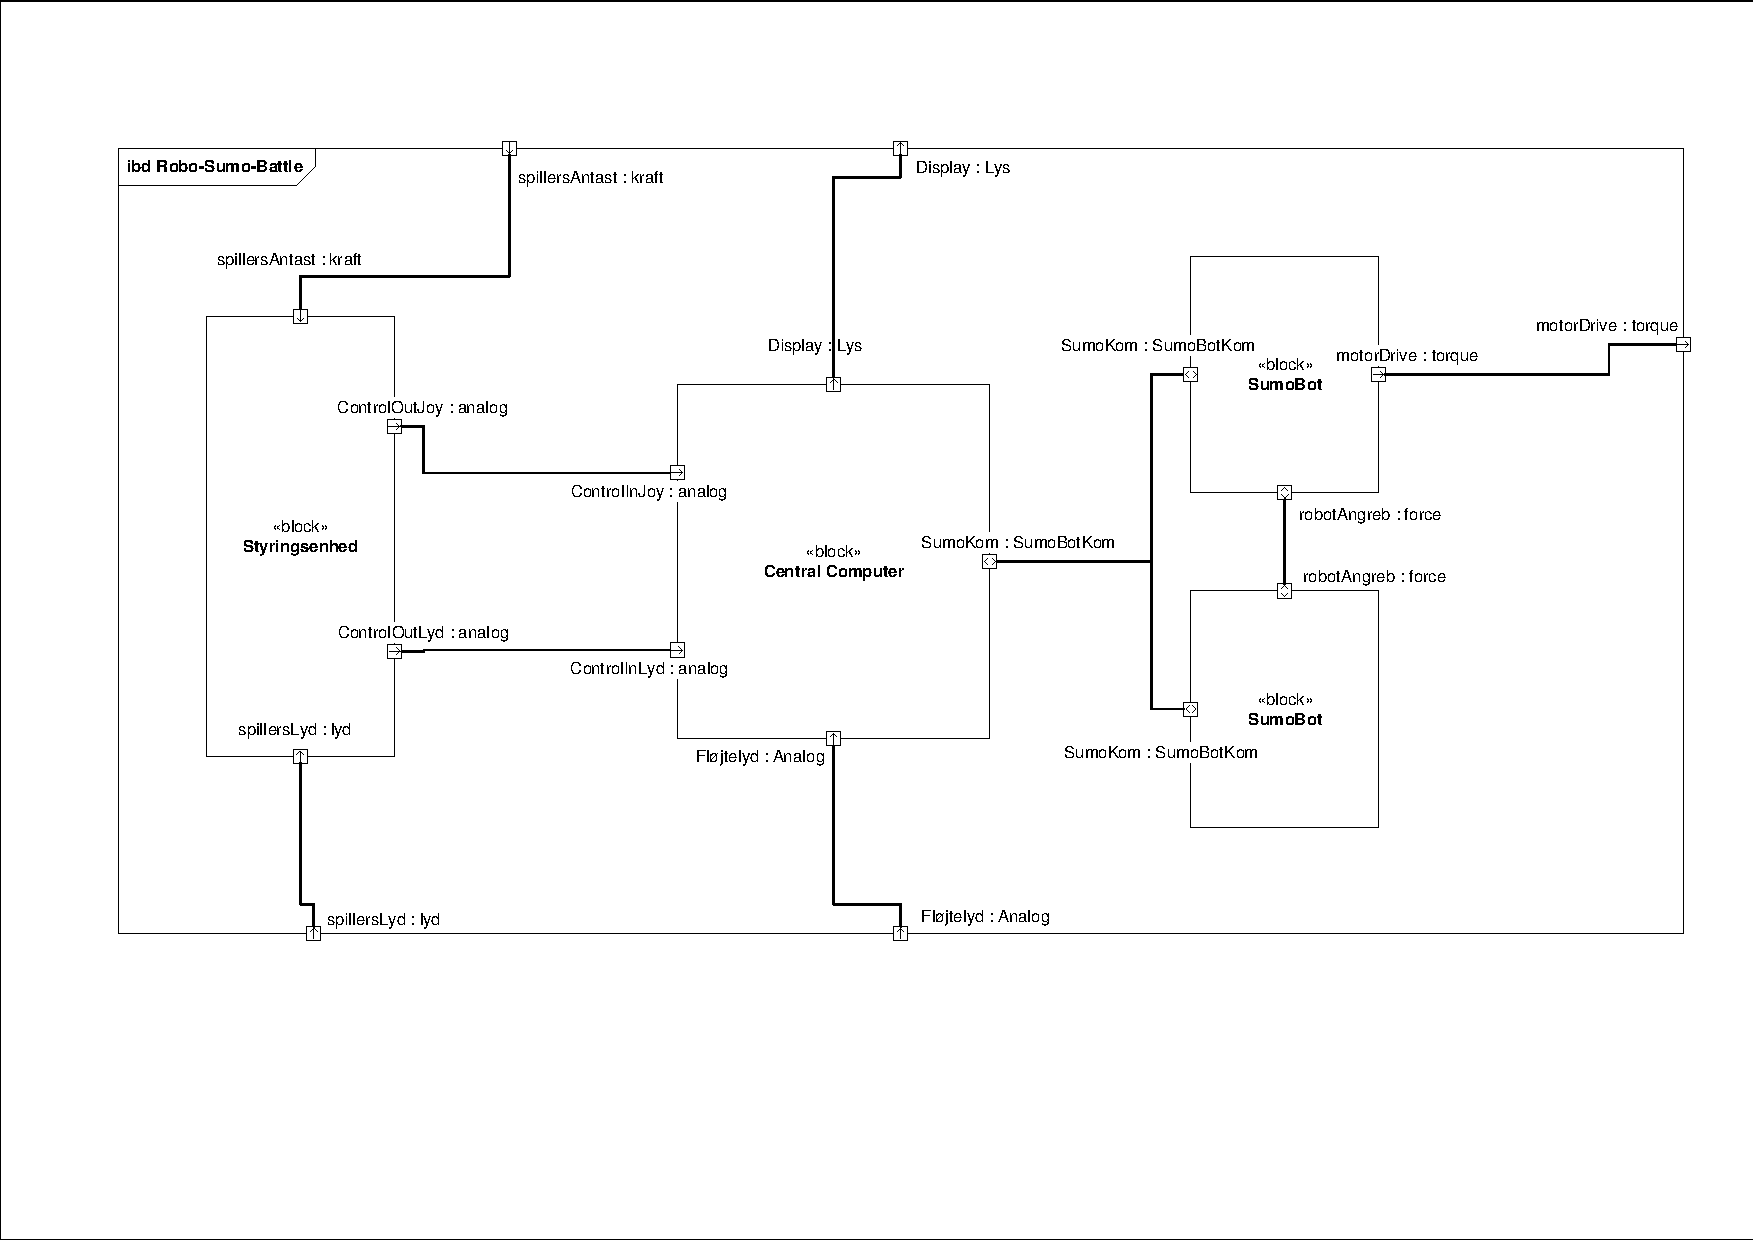
\includegraphics[page=1,width=1\linewidth]{figs/Diagrammer/IBD.pdf}
	\caption{System IBD}
	\label{fig:IBD_System}
\end{figure*}
\begin{figure*}
	\centering
   	\includegraphics[page=2,width=1\linewidth]{figs/Diagrammer/IBD.pdf}
	\caption{IBD for Styringsenhed}
	\label{fig:IBD_Styringsenhed}
\end{figure*}
\begin{figure*}
	\centering
   	\includegraphics[page=3,width=1\linewidth]{figs/Diagrammer/IBD.pdf}
	\caption{IBD for Central Computer}
	\label{fig:IBD_CentralComputer}
\end{figure*}

\begin{figure*}
	\centering
   	\includegraphics[page=4,width=1\linewidth]{figs/Diagrammer/IBD.pdf}
	\caption{IBD for SumoBot}
	\label{fig:IBD_SumoBot}
\end{figure*}

\subsection{Kontroller}
\subsubsection*{\textbf{Controller}}\hfill\\
Controller udgøre grænsefladen til den fysiske værden. Her konvertere force og lyd til data som bilkontrol kan læse og respondere på.
\subsubsection*{\textbf{Microcontroller}}\hfill\\
Microcontroller står for alt modtagelse af analoge signaler fra henholdsvis lydmodul og Joystick, oversætter det til data, som derfra sendes til Bilkontrold via transmitteren.
\subsubsection*{\textbf{Transmitter}}\hfill\\
Kommunikations portal til bilkontrol.
\subsubsection*{\textbf{ADC}}\hfill\\
Oversætter analoge signaler til digitale.
\subsubsection*{\textbf{Joystick}}\hfill\\
Joystic oversætter force til spændinger, som kan læses af microcontrolleren.
\subsubsection*{\textbf{Lyd-modul}}\hfill\\
Lydmodul konvertere lyd til analoge signaler som microcontrolleren kan evaluere på.
\subsubsection*{\textbf{Mikrofon}}\hfill\\
mikrofon gør det muligt for systemet at modtage lyd fra omverdenen.
\subsubsection*{\textbf{Analog filterbehandling}}\hfill\\
Analog filterbehandling filtrerer uønsket frekvenser modtaget fra mikrokrofonen og forstærker eller formindsker signalet, således det er læsbart for en mikrocontroller.



\subsection{Robot}

\figOC{Diagrammer/SumoBot_Bdd.png}{0.6}{System Blokdiagram over sumobot}

\subsubsection*{\textbf{Batteri}}\hfill\\
Forsyner vores system
\subsubsection*{\textbf{Motorstyring}}\hfill\\
Kontrollerer hastighed (vha. PWM) og rotationsretning via H-bro. Bliver styret af PSoC
\subsubsection*{\textbf{Motor}}\hfill\\
En DC-motor der roterer hjul efter en given hastighed og retning fra motorstyring
\subsubsection*{\textbf{PSU}}\hfill\\
Forsyner korrekt spænding til de enkelte delelementer i systemet
\subsubsection*{\textbf{RPi}}\hfill\\
Ansvarlig for den trådløse kommunikation mellem controller og PSoC.
\subsubsection*{\textbf{PSoC}}\hfill\\
Hovedstyringen for SumoBot. \\
Styrer motorstyring afhængig af signal fra RPI’en
Derudover modtager input fra attacksensor, der bearbejder disse til indikering af liv (afventer videre detaljer omkring spilregler)
\subsubsection*{\textbf{AttackSencor}}\hfill\\
Registrering af ”angreb”, som gives videre til PSoC.
\subsubsection*{\textbf{Scoreboard}}\hfill\\
En visuel indikering til brugeren af antal liv for de enkelte SumoBots

\subsection{Bilkontrol}


\subsubsection*{\textbf{Bilkontrol}}
Bilkontrollen er den centrale enhed som samler input fra controllere, sender signal til de to bots om retning og hastighed og styrer spillet. 
\subsubsection*{\textbf{Embedded controller}}
Bilkontrollens software eksekveres på en embedded controller med Linux-system. 
\subsubsection*{\textbf{Receiver}}
Receiver-modulet modtager serielt ikke-processeret input fra controllerens joystik og mikrofon via kabel. 
\subsubsection*{\textbf{Transmitter}}
Transmitter-modulet varetager den trådløse forbindelse til de to bots.
\subsubsection*{\textbf{Trådløs IF}}
Trådløse interface-modulet fungerer som undermodul til Transmitter-modulet og varetager den trådløse forbindelse til de to bots. 
\subsubsection*{\textbf{Digital lydbehandling}}
Digital lydbehandlings-modulet processerer mikrofonernes inputs således disse kan indgå i gameplayet som en styring til de to bots.  
\subsubsection*{\textbf{Gameplay}}
Gameplay-modulet varetager styring af spillets gang mv.  
\subsubsection*{\textbf{Point}}
Point-undermodulet til gameplay-modulet styrer spillernes point 
\subsubsection*{\textbf{Display}}
Display-undermodulet til gameplay-modulet viser kampens status igennem spillernes point. 
\subsubsection*{\textbf{Controller behandling}}
Controller behandlingsmodulet omsætter de ikke-processerede input fra controlleren (herved forstås input fra joystik og mikrofon) og omsætter dem til retning og hastighed for de to bots.  
\subsubsection*{\textbf{Joystick behandling}}
Joystick behandlingsmodulet omsætter det ikke-processerede input fra joystikket til retning og hastighed for de to bots.

\begin{figure*}
	\centering
   	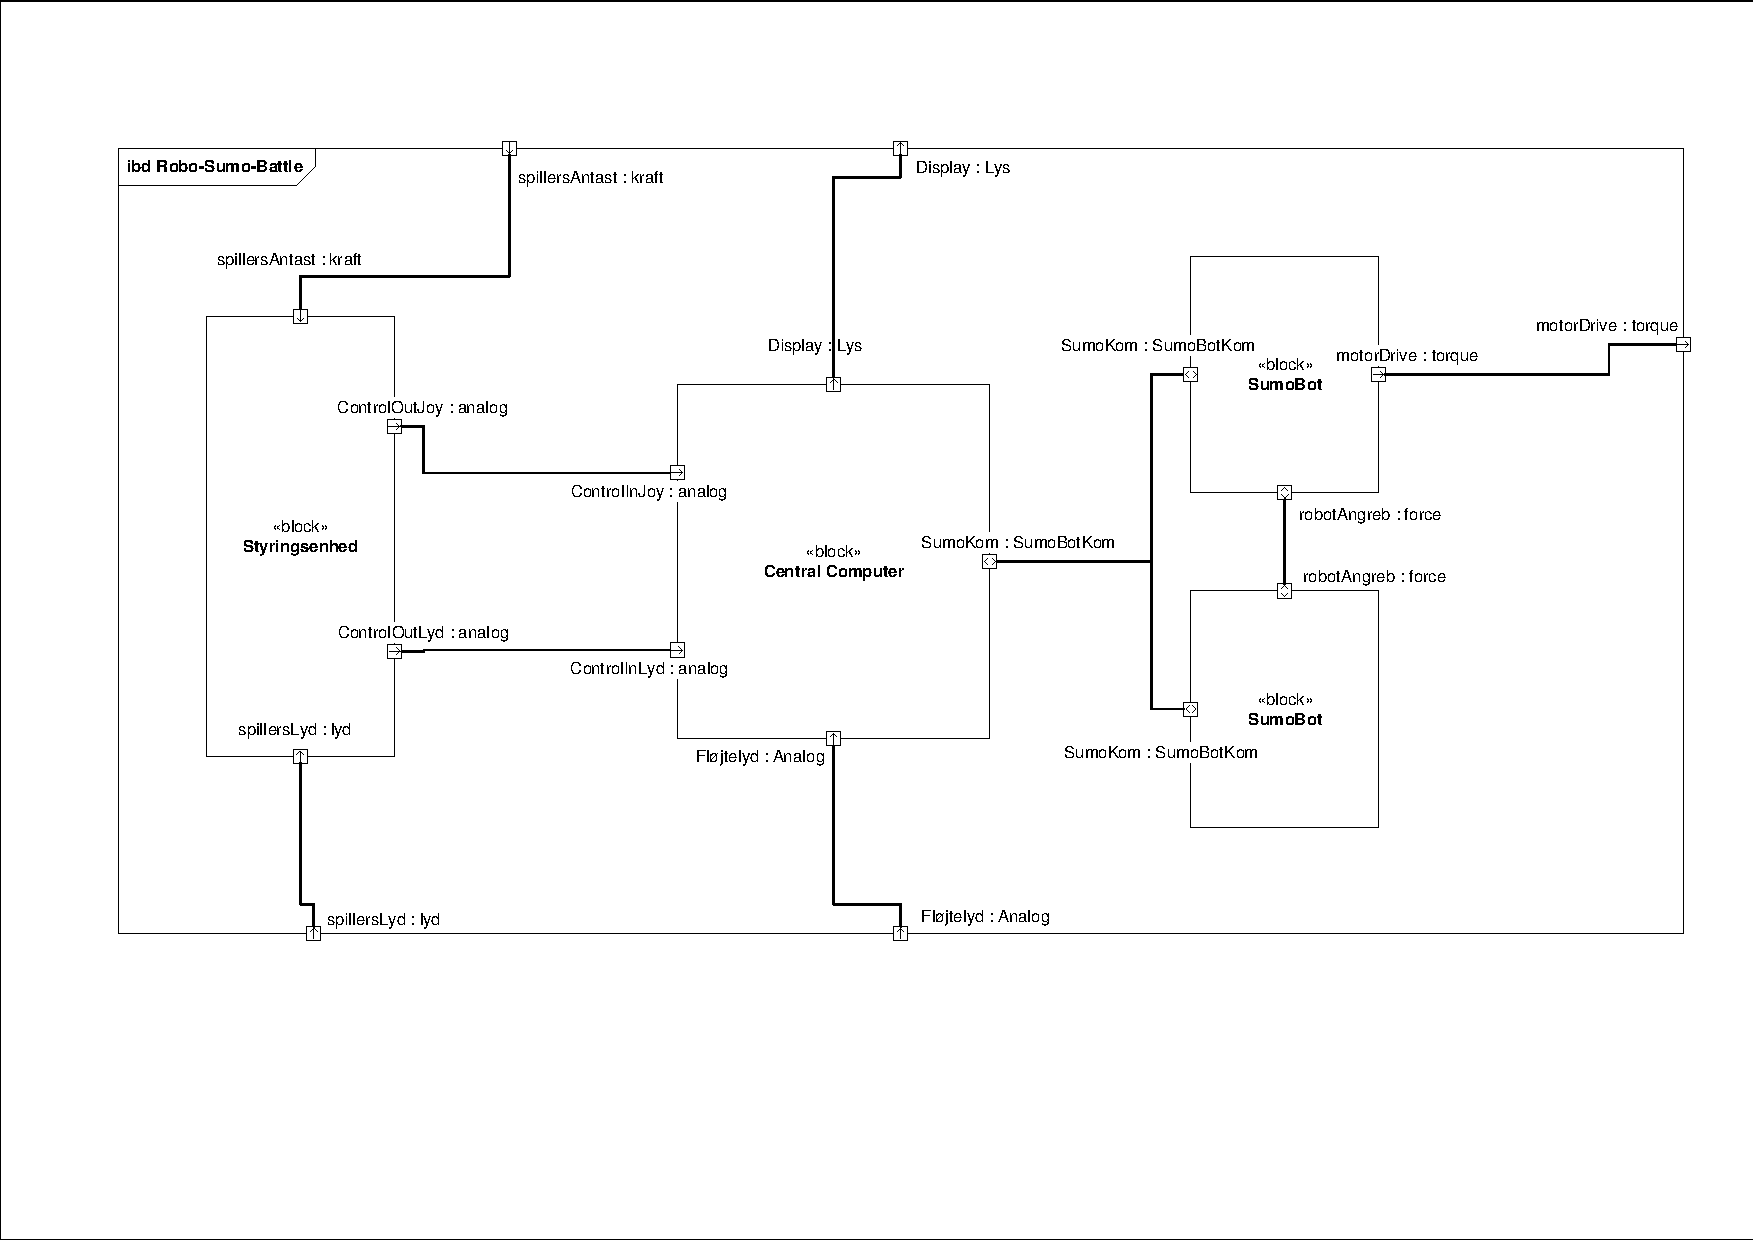
\includegraphics[page=1,width=1\linewidth]{figs/Diagrammer/IBD.pdf}
	\caption{System IBD}
	\label{fig:IBD_System}
\end{figure*}
\begin{figure*}
	\centering
   	\includegraphics[page=2,width=1\linewidth]{figs/Diagrammer/IBD.pdf}
	\caption{IBD for Styringsenhed}
	\label{fig:IBD_Styringsenhed}
\end{figure*}
\begin{figure*}
	\centering
   	\includegraphics[page=3,width=1\linewidth]{figs/Diagrammer/IBD.pdf}
	\caption{IBD for Central Computer}
	\label{fig:IBD_CentralComputer}
\end{figure*}

\begin{figure*}
	\centering
   	\includegraphics[page=4,width=1\linewidth]{figs/Diagrammer/IBD.pdf}
	\caption{IBD for SumoBot}
	\label{fig:IBD_SumoBot}
\end{figure*}

\subsection{Kontroller}
\subsubsection*{\textbf{Controller}}\hfill\\
Controller udgøre grænsefladen til den fysiske værden. Her konvertere force og lyd til data som bilkontrol kan læse og respondere på.
\subsubsection*{\textbf{Microcontroller}}\hfill\\
Microcontroller står for alt modtagelse af analoge signaler fra henholdsvis lydmodul og Joystick, oversætter det til data, som derfra sendes til Bilkontrold via transmitteren.
\subsubsection*{\textbf{Transmitter}}\hfill\\
Kommunikations portal til bilkontrol.
\subsubsection*{\textbf{ADC}}\hfill\\
Oversætter analoge signaler til digitale.
\subsubsection*{\textbf{Joystick}}\hfill\\
Joystic oversætter force til spændinger, som kan læses af microcontrolleren.
\subsubsection*{\textbf{Lyd-modul}}\hfill\\
Lydmodul konvertere lyd til analoge signaler som microcontrolleren kan evaluere på.
\subsubsection*{\textbf{Mikrofon}}\hfill\\
mikrofon gør det muligt for systemet at modtage lyd fra omverdenen.
\subsubsection*{\textbf{Analog filterbehandling}}\hfill\\
Analog filterbehandling filtrerer uønsket frekvenser modtaget fra mikrokrofonen og forstærker eller formindsker signalet, således det er læsbart for en mikrocontroller.



\section{Interne blokdiagrammer}
\begin{figure*}
	\centering
   	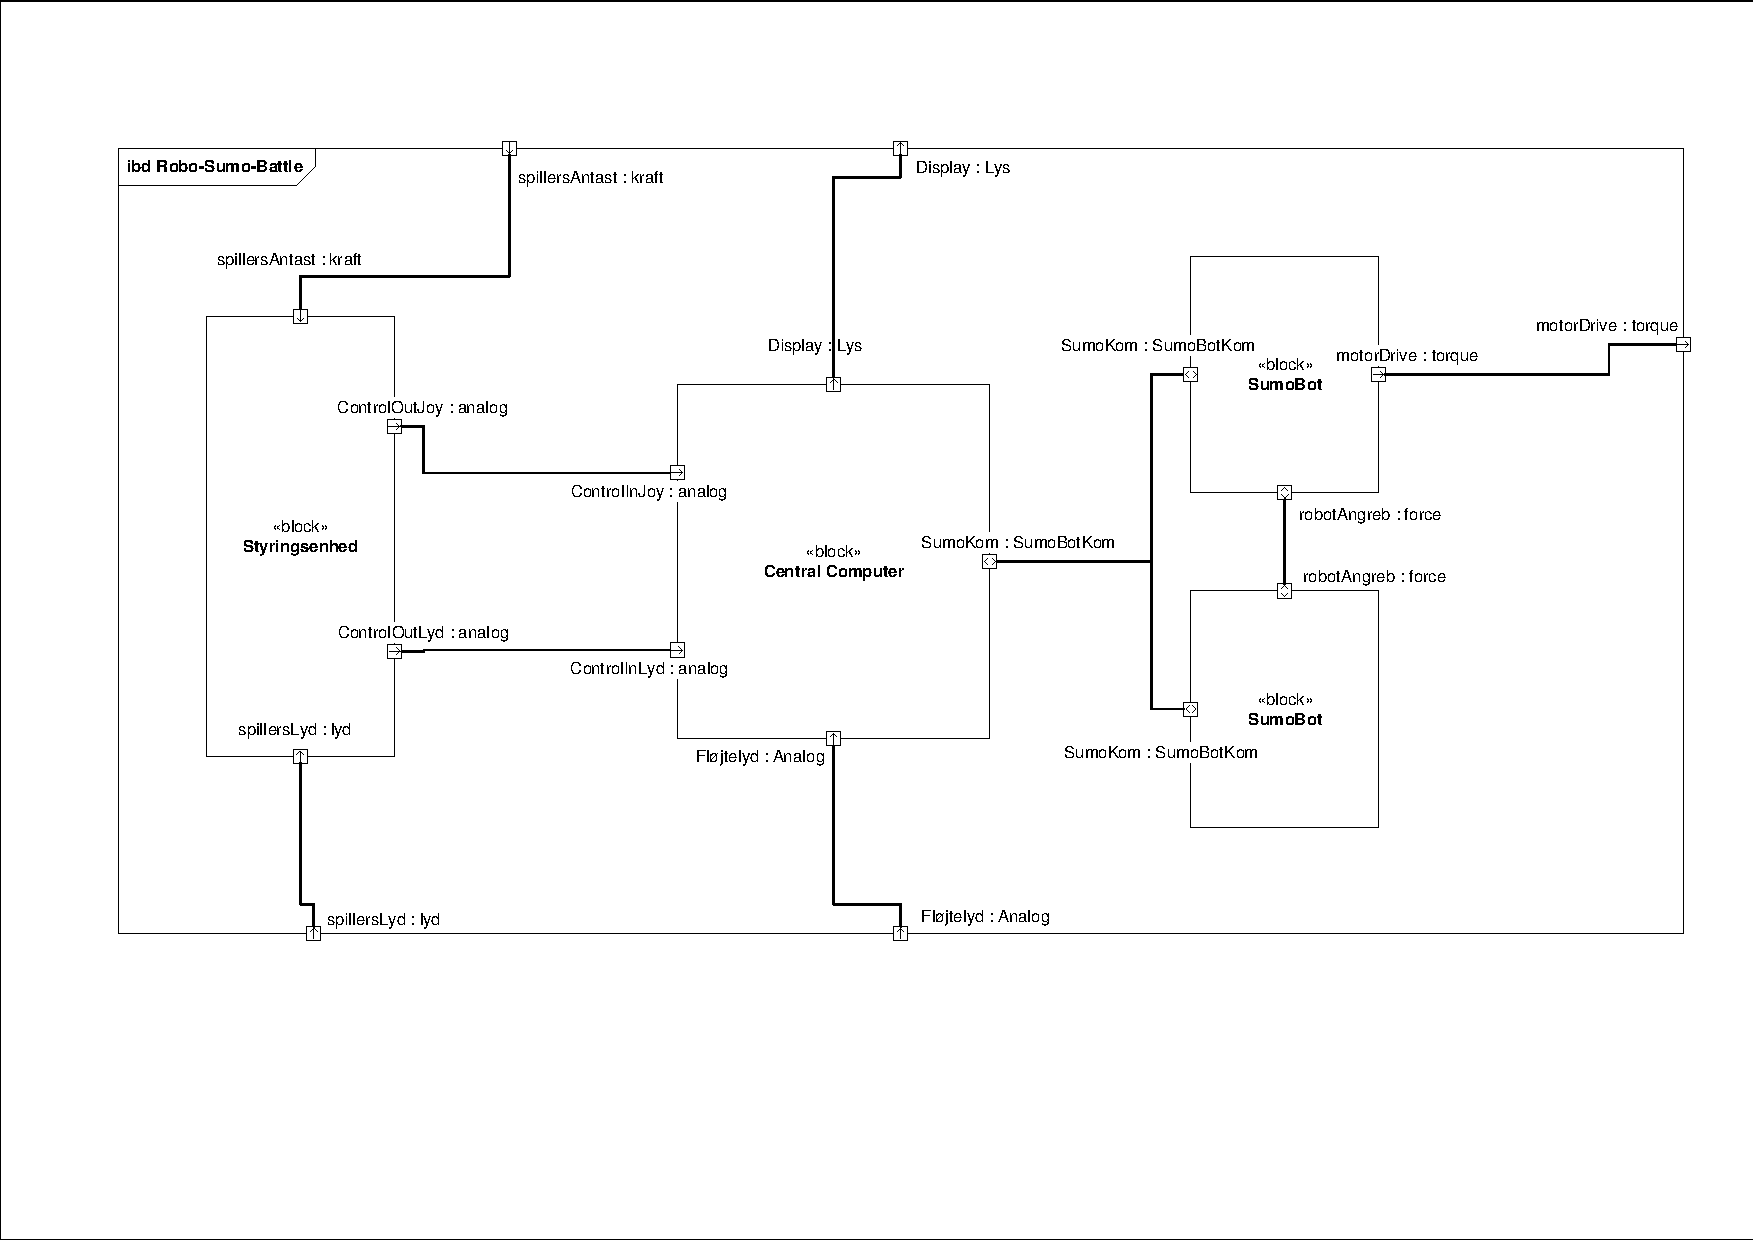
\includegraphics[page=1,width=1\linewidth]{figs/Diagrammer/IBD.pdf}
	\caption{System IBD}
	\label{fig:IBD_System}
\end{figure*}

\begin{figure*}
	\centering
   	\includegraphics[page=3,width=1\linewidth]{figs/Diagrammer/IBD.pdf}
	\caption{IBD for Central Computer, se \tabref{interface_table_CentralComputer} for interfacebeskrivelse}
	\label{fig:IBD_CentralComputer}
\end{figure*}
\begin{figure*}
	\centering
   	\includegraphics[page=2,width=1\linewidth]{figs/Diagrammer/IBD.pdf}
	\caption{IBD for Styringsenhed, se \tabref{interface_table_Styringsenhed} for interfacebeskrivelse}
	\label{fig:IBD_Styringsenhed}
\end{figure*}
\begin{figure*}
	\centering
   	\includegraphics[page=4,width=1\linewidth]{figs/Diagrammer/IBD.pdf}
	\caption{IBD for SumoBot, se \tabref{interface_table_SumoBot} for interfacebeskrivelse}
	\label{fig:IBD_SumoBot}
\end{figure*}

\subsection{Interface beskrivelser}
\noindent Der er udarbejdet en interface beskrivelse for de mere komplekse interfaces. For \figref{IBD_SumoBot} findes en dertilhørende interfacebeskrivelse i  \tabref{interface_table_SumoBot}.

\noindent For \figref{IBD_CentralComputer} findes en dertilhørende interfacebeskrivelse i \tabref{interface_table_CentralComputer}.
%%%%%%%%%%%%%%%%%
% 2020/10/24 - Adam
% Jeg har tilladt mig at "rydde" op i koden her, ved at tage udgangspunkt i UseCase.sty - Der er lavet et nyt environment \begin{SignalDescrption}{Navn}{label}
% Her i kan \signalbeskrivelse{navn}{type}{beskrivelse} skrives. - Se Grp6_tabels for mere info.
% Dette skulle gerne sikret et ensartet udtryk, samt et enkelt workflow. 
%%%%%%%%%%%%%%%%%
\begin{SignalDescription}{Central Computer}{CentralComputer}
    \signalbeskrivelse{in ctrlInJoy       }{Digital     }{Seriel forbindelse med defineret retning og hastighed}
    \signalbeskrivelse{in ctrlInLyd       }{Digital     }{Seriel forbindelse med defineret retning og hastighed}
    \signalbeskrivelse{out DisplayDataOut }{Digital Bus }{6 parallelforbindelser der overføre displayinformation}
    \signalbeskrivelse{out LCDOut         }{Light       }{Spilinformation til brugerne.}
    \signalbeskrivelse{inout robotKom     }{WIFI        }{Trådløs tovejskommunikation, til styring af SumoBot  og returnering af attacks }
\end{SignalDescription}

\begin{SignalDescription}{Styringsenhed}{Styringsenhed}
    \signalbeskrivelse{in ctrlInLyd    }{analog              }{\tbr Et lydsignal med frekvensindhold 100-10000 Hz}
    \signalbeskrivelse{in filterIn     }{analog              }{\tbr Lydsignal fra blokfløjte, muligvis overlejret med støj }
    \signalbeskrivelse{out joyStickOut }{                    }{\textbf{Bus med 5 signaler}:}
    \signalbeskrivelse{                }{1: analogX          }{spænding variende mellem 0 og VCC}
    \signalbeskrivelse{                }{2: analogY          }{spænding variende mellem 0 og VCC}
    \signalbeskrivelse{                }{3: digital          }{switch til at trykke på joystick controller}
    \signalbeskrivelse{                }{4:  VCC             }{5V}
    \signalbeskrivelse{                }{5: GND              }{0V}
    \signalbeskrivelse{out Mikrofon    }{analog              }{Udgangsimpedans 2,2k Ohm \tbr                               }
    \signalbeskrivelse{                }{                    }{Udgangsspænding 6,3 mV/Pa/1 kHz \tbr                        }
    \signalbeskrivelse{out ctrlOutJoy  }{analog              }{\tbr Samme som joyStickOut? Tilpasset i amplitude?          }
    \signalbeskrivelse{out ctrlOutLyd  }{\tbr analog/digital }{\tbr Interface til central computer                         }
\end{SignalDescription}
% \begin{table*}[]
%     \centering
%     \caption{Interfacebeskrivelse for Central Computer}
%     \label{tab:interface_table_CentralComputer}
%     \begin{tabular}{lp{5cm}p{7cm}}\toprule
%         Navn              & Type       & Beskrivelse\\                                                                                                                                 
%         in ctrlInJoy        & Digital    & Seriel forbindelse med defineret retning og hastighed\\
%         in ctrlInLyd        & Digital    & Seriel forbindelse med defineret retning og hastighed\\     
%         out DisplayDataOut  & Digital Bus     & 6 parallelforbindelser der overføre displayinformation\\
%         out LCDOut                & Light    & Spilinformation til brugerne.\\
%         inout robotKom       & WIFI              & Trådløs tovejskommunikation, til styring af SumoBot  og returnering af attacks\\
%         \bottomrule
%     \end{tabular}%
% \end{table*}

% \begin{table*}[]
%     \centering
%     \caption{Interfacebeskrivelse for Styringsenhed}
%     \label{tab:interface_table_Styringsenhed}
%     \begin{tabular}{lp{5cm}p{7cm}}\toprule
%         Navn              & Type       & Beskrivelse\\                                                                                                                                 
%         in ctrlInLyd      & analog     & \tbr Et lydsignal med frekvensindhold 100-10000 Hz\\
%         in filterIn       & analog     & \tbr Lydsignal fra blokfløjte, muligvis overlejret med støj\\                                                                                             
%         out joyStickOut   &            & Bus med 5 signaler:\\
%                           & 1: analogX & spænding variende mellem 0 og VCC\\                                                                                                        
%                           & 2: analogY & spænding variende mellem 0 og VCC\\                                                                                                            
%                           & 3: digital & switch til at trykke på joystick controller\\                                                                                                                
%                           & 4:  VCC    & 5V                                         \\                                                                                                      
%                           & 5: GND     & 0V                                         \\
%         out Mikrofon      & analog     & Udgangsimpedans 2,2k Ohm \tbr\\
%                           &            & Udgangsspænding 6,3 mV/Pa/1 kHz \tbr\\
%         out ctrlOutJoy & analog & \tbr Samme som joyStickOut? Tilpasset i amplitude?\\
%         out ctrlOutLyd & \tbr analog/digital & \tbr Interface til central computer\\                                                                                               
%         \\
%                 \bottomrule
%     \end{tabular}%
% \end{table*}
%%Sometimes it is a good idea to put domain objects in \texttt{}
%The template and the descriptions are based on the book Applying UML and Patterns: 
%An Introduction to Object-Oriented Analysis and Design and Iterative Development
%(3rd Edition) by Craig Larman.

%%% USE CASE 1
\subsubsection{Use Case 1}

\begin{usecase}
  \caption{Fully dressed beskrivelse af use case 1: "Styr \gls{sumobot} med joystick".}
  \addtitle{Use Case 1}{"Styr \gls{sumobot} med joystick"}
  %Level: "user-goal" or "subfunction"
  \addfield{Mål:}{At en \gls{sumobot} bevæger sig på spillebanen baseret på joystickinput.}
  %Level: "user-goal" or "subfunction"
  \addfield{Initiering:}{Spiller bruger joysticket som styringsenhed}

  %Primary Actor: Calls on the system to deliver its services.
  \addfield{Primær Aktør:}{Bruger}
  \additemizedfield{Sekundær Aktør:}{
    \item \gls{sumobot}
    \item Styringsenhed
    \item Central computer
  }

  \addfield{Antal samtidig forekomster:}{2}

  %Preconditions: What must be true on start and worth telling the reader?
  \addfield{Prækondition:}{\gls{rbs}-spillet er initieret \tbr}
  %when multiple
  %\additemizedfield{Preconditions:}{} 

  %Postconditions: What must be true on successful completion and worth telling the reader
  \additemizedfield{Postkonditioner:}{
    \item \gls{sumobot} har bevæget sig på baggrund af styringsinput fra joysticket.
    \item Afventer nyt input.
  }
  %when multiple
  %\additemizedfield{Preconditions:}{}

  %Main Success Scenario: A typical, unconditional happy path scenario of success.
  \addscenario{Hovedscenarie:}{
    \item Brugeren tilgår joystick-styringsenhed for spiller 1
    \item Brugeren bevæger joysticket
    \item Styringsenheden behandler bevægelsen
    \item[] [Ext01: Bruger styrer hastighed]
    \item[] [Ext02: Bruger styrer retning]
    \item Styringsenhed overfører data til central computer
    \item Central computer behandler styringsdata
    \item Central computer overfører styringsdata til \gls{sumobot}
    \item \gls{sumobot} udfører bevægelse.
  }
  \addscenario{Udvidelser / Undtagelser:}{
    \item[Ext01:] Bruger styrer hastighed
    \item[1.] Bruger tilter joystick på $y$-aksen.
    \item[2.] Use case fortsætter fra punkt 3\newline
    \item[Ext02:] Bruger styrer retning:
    \item[1.] Bruger tilter joystick på $x$-aksen.
    \item[2.] Use case fortsætter fra punkt 3
  }
\end{usecase}\label{tab:UseCase:1}
  - de driller- jeg fixer.
\section{Central Computer Analyse}

\subsection{Processor}
\textcolor{red}{Vi har nok behov for at tilføje en processor til BDD'et}
Til styringsenheden er behov for en processor, som opfylder følgende krav: 
\begin{itemize}
\item Skal kunne opbevare information om spillets status (liv, tid mv.) 
\item Skal kunne drive et Linux platform
\item Skal kunne agere access point for vores trådløse forbindelse 
\item Skal kunne behandle input fra styringsenhederne
\end{itemize}

Til denne del af systemet vil derfor blive brugt en Raspberry Pi Zero W, med en Linux distribution kaldet "Golden Ase" udviklet af Aarhus Universitet. Distributionen er en version af Linux distributionen Poky (V. 3.1.2 / Dunfell) og som er bygget på Linux Kernelen 5.4.51. Denne distribution gør det let at kommunikere gennem SSH med RPien og er veldokumenteret, uden behov for ekstra skærm. Golden Ase-distributionen er i øvrigt født med en websocket server. 
RPIen er dog ikke født med ADC, hvorfor inputtet til denne må være digitalt allerede fra styringsenheden. 

\subsection{Styringsenhed IF}
\textcolor{red}{Mangler afklaring}

\subsection{SumoBot IF}
Til at kommunikere med SumoBot skal der kortlægges både en passende teknologi og de første linjer for en protokol. 

\subsubsection{Teknologi}
Det er fastlagt gennem kravspecifikationen at vi skal bruge trådløs kommunikation, der som minimum skal kunne kommunikere på afstande >2-3 meter. Rasperry Pi er født med hardware som kan varetage kommunikation over både Bluetooth og Wifi. 
Både Wifi, Bluetooth og RF-kommunikation er blevet overvejet og RF-kommunikation er hurtigt blevet fravalgt grundet behovet for ekstra ekstra moduler tilkoblet vores RPi. Wifi er blevet valgt fremfor Bluetooth da det er en teknologi som gruppens medlemmer på forhånd er fortrolige med. Trådløs kommunikation er ikke et vigtigt læringsmål og ej heller et område som vi tidligere har beskæftiget os betydeligt med, hvorfor vi vil benytte os af frameworks i videst mulig udstrækning. 

\textbf{Forbindelse}\newline
Forbindelsen mellem Central Computer og SumoBot vil lavpraktisk basere sig på at Central Computer laver et access point (AP) ved opstart. Begge SumoBot vil ved opstart koble sig på dette access point og således have en direkte forbindelse til Central Computeren. 

\textbf{Kommunikationen}\newline
Kommunikationen vil foregå vha. websockets, hvor Central Computer vil agere server og SumoBot's vil agere clients - dette fordi det primært er Central Computer som skal give besked til SumoBot i form af kommandoer omkring hastighed og retning. Der vil dog også skulle kommunikeres fra SumoBot til Central Computer omkring angreb og hvorvidt en SumoBot har forladt banen. 

\subsubsection{Protokol}
Protokollen som beskriver retning og hastighed vil være en ganske simpel streng sammensat af retning og hastighed og vil blive defineret. 

\subsubsection{Trådløs Modul}
RPI Zero W er født med en bcm43438-chip som er fuldt understøttet af Linux og som vil blive benyttet til at lave access pointet. 

\subsection{Display}
Til at formidle antallet af resterende liv hos de to modstandere skal bruges et display. 

\textbf{LCD 16X2. HD44780 driver} \newline

https://www.circuitbasics.com/raspberry-pi-lcd-set-up-and-programming-in-c-with-wiringpi/


Fordele: 
\begin{itemize}
\item Der findes mange c-biblioteker til brugen af et LCD display. 
\item Der er mulighed for at vise små grafikker som ultimativt giver større nice-faktor
\item Skærmen kan vise 32 karaktere ad gangen.
\item Det er muligt at øge overføringshastigheden af data til skærmen, fra 4 bit til 8 bit ved at benytte yderligere 4 GPIO pins.
\end{itemize}

Ulemper: 
\begin{itemize}
\item Et standard LCD display benytter 6 GPIO's fra microprocessoren. 
\item Da der benyttes parallelkommunikation til LCD skærmen, og dermed bruges minimum 6 GPIO pins.
\end{itemize}

\textbf{7-segment}
Fordele: 
\begin{itemize}
\item Vi har erfaring med brug af 7-segmentsdisplay
\item Der er et relativt småt strømforbrug ved brug af 7-segmentsdisplay 
\end{itemize}

Ulemper: 
\begin{itemize}
\item Der er en lille nice-faktor ved brug af 7-segmentsdisplay. 
\item 7-segmentsdisplayet skal bruge 10 forbindelser (5 ved brug af std. driver)
\item Der skal benyttes ihvertfald 2 x 7-segments displays hos hver modstander = 4 stk. total, hvilket kræver mange forbindelser. 
\end{itemize}

\textbf{LED} \newline
Fordele: 
\begin{itemize}
\item Det er enormt simpelt at tænde og slukke LED's forbundet til GPIO's
\item Det er nemt at se på afstand hvor mange resterende liv hver modstander har
\end{itemize}

Ulemper: 
\begin{itemize}
\item Det er svært at demonstrere resterende tid på en intuitiv måde
\item Brugen af GPIO's bliver høj
\item Igen er nice-faktoren ekstrem lav ved brug af LED'er
\end{itemize}

\subsubsection{Konklusion}
I denne del af systemet vægtes nice-faktoren højt, da displayet kommer til at få stor opmærksomhed fra både spillere og tilskuere. Det vægtes også højt at brugen af GPIO's er begrænset. Derfor besluttes at benytte LCD displayet af typen \textit{'LCD 16X2. HD44780 driver'}. Der er en mindre risiko forbundet med brugen af LCD-displayet da vi ikke tidligere har brugt dette, men til gengæld er der meget information at hente på nettet omkring brugen af dette specifikke display. 

\subsubsection{Point-Modul}
\textcolor{red}{Simon: Dette modul virker ikke til at være et hardware modul. Nogle indsigelser mod at fjerne det?} 
\section {Styringsenhed analyse}
%% Analysis without numbers is just opinions.
\subsection{Mikrofon}
\begin{itemize}
    \item Skal være i stand til at opfange frekvenser i det hørbare område\footnote{\SIrange{20}{20e3}{Hz}}. 
    \item Må ikke afvige i måling hvis samme tone/frekvens spilles til den. 
\end{itemize}

Som mikrofon har vi tænkt os at benytte os af en "electret microphone"\cite{CompleteECMGuide}\cite{MCE4500Datasheetb} \footnote{\url{https://bekent.dk/mce-4500.html?gclid=Cj0KCQjwuL_8BRCXARIsAGiC51A8KKsYBFYi-5kmvFSPHIzzuJ2TXDr6Rnnl_QvKquKd7tBmXM7CuLgaAiHaEALw_wcB}}.
Der er en risiko forbundet hertil, at den simpelthen ikke er præcis nok til konsistent at gengive frekvenser rimeligt, så der kan laves lydbehandling af den til en protokol til at styre robotterne. 
En fordel er, at det er en simpel kondensator mikrofon, og vi i MSE har lært at designe forstærkere til kapacitive inputs.
Dertil også, at vi selv kan modificere inputtet med de filtre af eget valg.

\subsection{Analog filterbehandling}
\begin{itemize}
    \item Skal filtrere signalet fra netstøj og HF-støj før forstærkning. 
\end{itemize}

Her er et hav af muligheder for forskellige implementeringer. Som udgangspunkt vægter vi intet ripple i pasbåndet med ripple i stopbåndet til følge. Vi har vurderet, at det er mest risikabelt med ripple i pasbåndet. /tbr %(ikke enig i at vi vægtede noget)
\fig{Analyse/FilterResponse_AOE_f-6-30}{1}{%
\emph{Normalized frequency response graphs for the 2-, 4-, 6-, and 8-pole filters in Table 6.2. The Butterworth and Bessel filters are normalized to 3dB attenuation at unit frequency, whereas the Chebyshev filters are normalized to 0.5 dB and 2dB attenuations. As explained earlier, the top of the ripple band in the Chebyshev plots has been set to unity.} Figur lånt fra The Art of Electronics \cite[fig.~6.30]{Horowitz2015}}




Præcis hvilken type filter og orden studeres nærmere i designfasen. Dog viser flere kilder at et MFB filter er velegnet i en ADC forbindelse \cite[s.~413]{Horowitz2015}
En fordel ved at vælge et MFB-filter er den store dæmpning i stopbåndet, set i forhold til andre filtertyper\cite{ADCMFBTI}. Desuden findes en række applikationsnoter hvori MFB-filtre bruges i et ADC-konvertingsled. bruges\cite{OPA344Data}\tbr
\fig{Analyse/MFB_bode_AOE_f-6-37}{1}{%
\emph{The stopband attenuation of the MFB configuration is not much affected by rising op-amp output impedance (e.g., as seen in Figure 4.53), compared with that of the VCVS. However, you can mitigate the effect in the VCVS by using a second op- amp to create a buffered output from the signal at the op-amp’s noninverting input.} Figur lånt fra The Art of Electronics \cite[fig.~6.37]{Horowitz2015}}
\subsection{Spændingsforstærker}
\begin{itemize}
    \item Skal forstærkere spændingen op til et niveau hvor en ADC kan registrere dette og konvertere til kvanticerede bits.
    \item Skal have en stabil strømforsyning.
    \item Lav S/N ratio, \tbr skal defineres
    \item 100gg forstærkning \tbr
\end{itemize}
Generelt for de analoge kredsløb er der en risiko i, at strømforsyningen skal være meget stabil, da denne bruges som referencespænding til både signalet fra joysticket og mikrofonen. Altså betyder en afvigelse eller transient i strømforsyningen en afvigelse i kommandoen til robotterne, og man kan ikke vide sig sikker på om man er dårlig til spillet eller om strømforsyningen der sender transienter ud i kommandoprotokollen. 


\subsection{ADC}
\begin{itemize}
    \item \tbr Opløsning?
\end{itemize}
\tbr Afhængig af om interfacet fra styringsenheden til central computer skal være analog eller digital, skal det analoge signal fra styringsenheden digitaliseres. 
Der er en stor risiko i at designe ADC'erne selv, da der så skal tages hensyn til synkronisering af clocks m.m. Derfor vælges enten:
\begin{itemize}
    \item et ADC board til RPi med op til 6 inputs (hhv. 2x joystick til X retning, 2x joystick til Y retning samt 2x mikrofon)
    \item en mindst 6 kanals ADC (reference mcp3008) og så overføre dets output serielt til RPi på centralcomputeren, som så skal eksekvere kommandoer til SumoBots'ne på baggrund af dette. 
\end{itemize}

Derfor har vi fundet et ADC board til vores Raspberry Pi Zero: \footnote{\url{https://www.abelectronics.co.uk/p/69/adc-pi-raspberry-pi-analogue-to-digital-converter}}. Fra ADC'en er der serielt interface, således disse data kan sendes til en device (central computer IF), hvor der kan laves digital signalbehandling på dataen. Dette lader sig gøre med, at man kan generere C kode ud fra Matlab. Ellers findes der også veldefinerede biblioteker til ovenstående ADC board. 

\subsection{Central Computer IF}
\begin{itemize}
    \item blabla
\end{itemize}
data fra adc herind .. device applikation fra matlab eller bibliotek i Arduino???

\input{TeX/Formalia/SumoBotanalyse}
\bibliographystyle{IEEEtran}
\bibliography{biblo}
\end{document}

